\chapter{绪论}
\label{chap:Intro}
\section{题目背景介绍}
\subsection{并行计算}

Gordon Moore在1965年所做的预言在很长的一段时间内都被证明是准确的。在这个趋势下,CPU的性能基本每两年可以翻一番\cite{book:computer_architecture} 。这种快速的增长一度对于用户以及软件开发者而言意味着,要获得更快速的计算更好的性能,他们只需要等待下一代的微处理器带来的翻倍性能即可。但是自从2002年开始,单核处理器的性能增长就已经以每年20\%的速度下降~\cite{book:intro}。并且,在2005年之后,主要的微处理器制造商都一致认为未来处理器性能增长的出路在于并行化。与其尝试着突破散热和晶体管密度等的物理限制继续研究制造快速的单核处理器,制造商们纷纷尝试将多个可用的通用核集成到一个片上系统中。

这个重大改变对于一直享受“免费午餐”的软件开发者而言意义重大:从单核向多核的转变意味着不可能在对已有的串行软件毫无修改的情况下移植到多核平台还能立即享受多核带来的性能提升。以前的软件无法自己意识到多个核心的存在,在这样的平台上运行的程序的性能最多只能和运行在单核上一样,甚至运行性能更差。

至此,并行计算不仅仅存在于学术研究领域,更快速爆发地进入了工业界的每个角落。并行计算不仅仅调动着硬件开发者的生产力,也让众多的软件开发者参与其中,围绕并行计算、高性能计算等主题提出了众多的并行算法、编程模型以及开发平台,并且以此为基础,进一步提出了例如云计算、大数据等新的概念与模型。

可以说,并行计算已经从数十年前针对特殊应用的解决方案,变成了当今计算机领域的另一块基石,也因此,对于并行计算软硬件的研究也变得意义非常。

\subsection{并行软硬件的发展}\label{sec:progress}
一般而言,我们可以从结构模型、访存方式以及互联网络三个方面讨论并行计算机硬件的特征\cite{book:chen}。

并行计算领域常常引用弗林分类对计算机根据其数据流和指令流的数量划分为4类\cite{book:chen}。分别是单指令流单数据流(Single Instruction Single Data,SISD), 单指令流多数据流(Single Instruction Multiple Data, SIMD), 多指令流单数据流(Multiple Instruction Single Data,MISD)以及多指令流多数据流(Multiple Instruction Multiple Data,MIMD)。其中MISD结构目前还没有成熟的产品,MIMD和SIMD是当今比较常见的多核平台的架构。

另外,根据CPU访问内存的方式也可以对并行计算机进行分类。在规模较小的,一般为2~100个核之间的多核架构,通常采用共享内存的架构,即每个计算单元或者CPU都可以访问同一块内存,并且较小的核数可以保证每个核都可以以相同的速度访问内存的任意地址,这种方式称为均匀存储访问模型(Uniform Memory Access,UMA)。但是当核数增加,内存面积扩大之后,访问距离计算单元(核)较近的内存和访问较远内存的延迟将出现细微的差距,或者物理上内存是分布在各个处理单元内部,每个单元节点通过网络相连然后所有局部内存构成一个全局内存,这种情况下的内存访问模型就是非均匀的,称为非均匀存储访问模型(NonUniform Memory Access, NUMA),在非均匀存储访问模型中,如果保证缓存一致性,则被称为缓存一致的非均匀存储访问模型(cache coherent-NUMA, cc-NUMA)。

最后,可以根据连接多个处理器或者连接处理器与内存之间的网络对并行计算机进行分类。根据今年来对多处理器平台上的片上网络(Network on Chip, NoC)的研究和总结\cite{jour:NoC},现在的片上网络实现存在多种方案,主要的有点到点结构、Fat-tree结构、结构总线、星形结构、环状网络以及Mesh网络为主,其中Mesh网络在05年以后的架构中越来越常见。

并行硬件已经进入了我们的生活,现在几乎所有的台式电脑和服务器都使用的是多核处理器。然而,并行硬件似乎并没有跟上硬件的发展速度。除了一些操作系统、Web服务器以及数据库系统外,很少有多核应用见诸市面。正如上一小节所言,现有的串行软件不能自主地利用多核的优势,软件开发者想要继续提升性能,就必须适应并且熟悉现在的分布式内粗怒或者共享内存架构。

在共享内存架构,一般采用如下方式:程序以一个进程的方式启动,在需要并行处理的地方开启多个线程。这种以线程为基础的并行编程方式的一个代表是OpenMP和POSIX Thread,我们将在~\ref{chap:model-cmp}中进一步研究和讨论。另外,如果我们运行的是分布式内存的应用程序,一般都采用多个进程协作的方式,基于进程的并行编程方式的代表则为MPI和本文的核心OpenSHMEM。

随着众核处理器架构的出现在高性能计算领域,相关的并行编程模型,工具以及库的开发比以往任何时候都备受重视。

以往的并行计算领域基本只关注以MPI为代表的消息传递编程模型,或者是以OpenMP为代表的共享内存模型,但是由于PGAS的抽象模型以及它能够构建的一个直接清晰的内存访问和通信模型,最近对于部分全局地址空间(Partitioned Global Address Space,PGAS)的研究越来越多。现在比较有名的基于PGAS模型的语言或者库包括Unified Parallel C(UPC), X10, Chapel,Co-Array Fortran(CAF), Titanium, 以及SHMEM\cite{site:shmem_api}。

\subsection{并行技术的应用场景} 
数十年来,我们的生活在技术的推动下有了天翻地覆的变化,我们在享受这些变化的同时又成为了技术发展的直接推动力。我们现在正在进行的或者正在享受成果的一些项目,比如人类基因组项目,医学成像技术,Web的发展甚至是越来越精细的电影特效都是建立在快速发展的技术带来的计算性能飞跃的基础上的。 但是,我们要解决的问题似乎并没有随着性能翻番而减少,一些以前认为不可能的问题都亟待解决,要解决这些问题,就需要并行计算。以下是一些例子:
\begin{itemize}
\item 天气预报。要更精确的预测天气和气候的变化,就需要更为精确的模型,由于预测需要考虑众多的气象、大气、海洋等的因素,更为精确的模型意味着更多的计算量,这样的计算量即使在最先进的单核上也是无法想象的。
\item 模型模拟。科学计算一直是并行计算的最大“雇主”。在科学计算的领域,很多模型的验证需要大量的资金投入,有的甚至无法在现实中完成实验,这时就需要在计算机上进行模拟实验。而要在计算机中建立接近真实的模型,就需要大量的参数,随之而来的是大量的计算任务。最早的并行计算机就是在这样的驱动力下研究出来,目前为止,美国NASA依然是世界上最为著名的并行计算的主要支持者。
\item 数据分析。从计算机发展以来,尤其是互联网时代的到来,整个社会产生了巨大的数据量,然而如果不分析这巨大数据量背后的信息,这些巨量的数据都是无用的。比如人类的DNA,比如将要到来的物联网时代的传感信息,甚至是当今的云计算的海量数据存储和检索等等,都需要以并行计算为基础进行。
\end{itemize}
\section{国内外研究现状}
SIMD的编程方法对于大型并行系统而言比较适合,目前有许多不同的遵循SIMD的编程模型,比如Active Messagepassing(AM),分布式共享内存,以及PGAS~\cite{jour:tshmem}。在~\ref{sec:progress}部分中,我们提到了本文的主题,OpenSHMEM项目。OpenSHMEM项目虽然是在2011年被提出并成立,但实际上SHMEM编程模型在之前就存在了\cite{site:openshmem_spec}\cite{site:shmem_api}\cite{book:encyclopedia_of_parallel_computing}。但是由于多个厂商提供了几个不同版本的SHMEM实现,虽然遵循了一样的通信模型和思想,但是在一些调用细节上有所差异,导致SHMEM的各个实现之间的不可移植性,限制了SHMEM的发展。在众核平台开始兴起之后,由于PGAS模型被认为在大型多核平台上会有良好的表现,对于SHMEM的研究和热情重新被燃起,于是SHMEM的标准化工作被提出,即OpenSHMEM项目。以下对OpSHMEM和SHMEM项目的几个方面的研究现状逐一叙述。
\subsection{PGAS}
PGAS是一种同时适合于共享内存和分布式内存并行计算机的编程模型,这种计算机一般由几百甚至上千的CPU构成。一般PGAS的语言或者实现都具有以下特点:
\begin{enumerate}
\item 包含一组处理器,每个处理器都有自己的本地存储。每个本地存储的一部分被声明成是私有的,也就是无法被外部处理器所访问。
\item 一种共享机制,可以让每个处理器的存储的至少一部分与其他处理器共享。共享机制可以通过网络连接和软件实现,也可以通过保证缓存一致性的硬件共享内存实现。
\item 每个共享内存的地址有一个affinity处理器,指的是内存位于该处理器的本地内存区域,所以这个处理器访问该内存的延迟最小。
\end{enumerate}
目前支持PGAS的语言有很多\cite{book:encyclopedia},比较广泛的有UPC,X10以及Titanium等。此外,对于PGAS模型的支持软硬件研究,PGAS模型的优势研究等也在进行中\cite{jour:NIC}。
\subsection{SHMEM与GSHMEM,TSHMEM}
SHMEM通信库最早是由Cray公司为他们的T3D系统以及T3E模型系统所做的应用程序接口。这些系统通常包括了一个逻辑上共享内存地址空间,而物理上却是分布式存储的内存子系统,并且包含一个内存互联网络,一组处理单元(Processing Elements,PEs),一组I/O网关以及一个host子系统。这两个系列的系统可以支持一些延迟隐藏机制,比如预取机制,远程存以及块转换引擎(Block Transfer Engine,BLT)。

SHMEM后来被SGI采用,移植到SGI基于Numa-Link架构的产品上去,并且包含在了消息传递工具箱(Message Passing Toolkit)中。以后的SHMEM实现基本都是从SGI的版本演化而来。现有的SHMEM API支持C,C++以及Fortran语言\cite{site:openshmem_spec}。

在OpenSHMEM之前,关于SHMEM的工作大多与平台相关,并且稍有区别。在OpenSHMEM标准化说明文档发布之后,除了主页放出的实现样例,还有佛罗里达大学所做的GSHMEM实现\cite{jour:gshmem}。GSHMEM是GatorSHMEM的简称,是一个面向大型服务器的OpenSHMEM实现。GSHMEM采用GASNet作为通用的网络通信层,将大量的管理和通信任务交给成熟稳定的GASNet来完成。并且在GSHMEM的实现中,还参考了MPI的接口的使用情况,建议增加并且实现了两个新的接口,gather和scatter。

随后,在2012年,佛罗里达大学实现了TSHMEM\cite{jour:tshmem}。TSHMEM是TileraSHMEM的简称。TSHMEM是在Tilera众核平台上的OpenSHMEM实现。TSHMEM的实现借鉴了GSHMEM的工作,但是这次没有采用GASNet,而是直接调用了Tilera提供的网络通信接口。

除了这些在新平台上重新实现OpenSHMEM的工作,还有一部分工作思路是采用新的映射方法,在原有的平台或者操作系统上提供对OpenSHMEM的支持\cite{jour:intra-node}。
\subsection{GASNet}
在OpenSHMEM主页放出的样例以及GSHMEM的实现中,都采用了GASNet作为较底层的网络通信层,如图~\ref{fig:gasnet}。GASNet是Global-Address Space Networking的简称,本身是语言无关的底层的网络层,是加州大学伯克利分校和劳伦斯伯克利国家实验室(LBNL)于1993年联合实现。GASNet提供了网络无关的高性能通信原语,支持SPMD并行编程模型,尤其对PGAS类型的语言和库有直接的支持。

总的看来,GASNet分为两层,分别是GASNet核心API以及GASNet扩展API。其中核心API实现在不同的网络接口上,而扩展API则是完全网络无关的,提供中级或者高级抽象的网络通信操作接口。并且有的扩展API是直接实现在互联层API上的,因此在可能的地方,GASNet可以支持RMDA来提高性能。
\begin{figure}
\centering
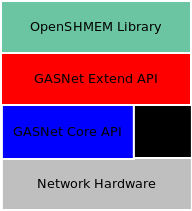
\includegraphics{gasnet_layer.png}
\caption{GASNet和OpenSHMEM的层次结构}\label{fig:gasnet}
\end{figure}
目前,GASNet可以支持在一系列常见的网络上运行,比如UDP,MPI,Cray XT Portals等等。

\subsection{Tilera众核平台}
Tilera公司,坐落于加州San Jose,是一家以设计以及开发商用众核处理器的公司,Tilera的产品着重强调了高性能和低功耗,因此在云计算、通用服务器以及嵌入式设备市场上十分流行。

每个Tilera的众核处理器都是一个可扩展的二维Mesh网络的连接结构,每个核被称为tile,每个tile中包含了一个处理器核新,以及私有的cache系统,cache系统可以通过片上网络和内存互联,这种技术被称为iMesh。Tilera的可扩展二维Mesh网络由提供数据路由的动态网络构成,数据可以在内存控制器、缓存以及外部I/O之间传递交换,开发者可以通过调用Tilera提供的通信原语控制数据的传输。

\section{研究方法与设计思路}
本文的安排如下。第一部分绪论,大致叙述了目前并行计算的发展情况,对并行计算的软硬件发展以及目前流行的几种编程模型做一简述,并且总结有关OpenSHMEM和SHMEM相关的工作。第二部分,作为对一个较不熟悉的编程模型的研究,首先先将其和其他几种常见的编程方法做一比较,然后根据OpenSHMEM的特性说明OpenSHMEM为什么会重新受到关注。第三部分,简述并行程序设计的基础准则,之后用OpenSHMEM实现一个矩阵乘法的例子说明OpenSHMEM编程的原则,随后对于并行计算中最重要的议题,性能优化做一研究。在最后一个部分中,简述了Tilera-Gx8036平台的平台特性,并且尝试在该平台上实现OpenSHMEM API的一个功能子集。